\documentclass[onlymath]{beamer}
% \documentclass[onlymath,handout]{beamer}

% Macros used by all lectures, but not necessarily by excercises

%%% General setup and dependencies:

% \usetheme[ddcfooter,nosectionnum]{tud}
\usetheme[nosectionnum,pagenum,noheader]{tud}
% \usetheme[nosectionnum,pagenum]{tud}

% Increase body font size to a sane level:
\let\origframetitle\frametitle
% \renewcommand{\frametitle}[1]{\origframetitle{#1}\normalsize}
\renewcommand{\frametitle}[1]{\origframetitle{#1}\fontsize{10pt}{13.2}\selectfont}
\setbeamerfont{itemize/enumerate subbody}{size=\small} % tud defaults to scriptsize!
\setbeamerfont{itemize/enumerate subsubbody}{size=\small}
% \setbeamerfont{normal text}{size=\small}
% \setbeamerfont{itemize body}{size=\small}

\renewcommand{\emph}[1]{\textbf{#1}}

\def\arraystretch{1.3}% Make tables even less cramped vertically

\usepackage[ngerman]{babel}
\usepackage[utf8]{inputenc}
\usepackage[T1]{fontenc}

%\usepackage{graphicx}
\usepackage[export]{adjustbox} % loads graphicx
\usepackage{import}
\usepackage{stmaryrd}
\usepackage[normalem]{ulem} % sout command
% \usepackage{times}
\usepackage{txfonts}
\usepackage{array}

% \usepackage[perpage]{footmisc} % reset footnote counter on each page -- fails with beamer (footnotes gone)
\usepackage{perpage}  % reset footnote counter on each page
\MakePerPage{footnote}

\usepackage{tikz}
\usetikzlibrary{arrows,positioning,decorations.pathreplacing}
% Inspired by http://www.texample.net/tikz/examples/hand-drawn-lines/
\usetikzlibrary{decorations.pathmorphing}
\pgfdeclaredecoration{penciline}{initial}{
    \state{initial}[width=+\pgfdecoratedinputsegmentremainingdistance,
    auto corner on length=1mm,]{
        \pgfpathcurveto%
        {% From
            \pgfqpoint{\pgfdecoratedinputsegmentremainingdistance}
                      {\pgfdecorationsegmentamplitude}
        }
        {%  Control 1
        \pgfmathrand
        \pgfpointadd{\pgfqpoint{\pgfdecoratedinputsegmentremainingdistance}{0pt}}
                    {\pgfqpoint{-\pgfdecorationsegmentaspect
                     \pgfdecoratedinputsegmentremainingdistance}%
                               {\pgfmathresult\pgfdecorationsegmentamplitude}
                    }
        }
        {%TO
        \pgfpointadd{\pgfpointdecoratedinputsegmentlast}{\pgfpoint{1pt}{1pt}}
        }
    }
    \state{final}{}
}
\tikzset{handdrawn/.style={decorate,decoration=penciline}}
\tikzset{every shadow/.style={fill=none,shadow xshift=0pt,shadow yshift=0pt}}
% \tikzset{module/.append style={top color=\col,bottom color=\col}}

% Use to make Tikz attributes with Beamer overlays
% http://tex.stackexchange.com/a/6155
\tikzset{onslide/.code args={<#1>#2}{%
  \only<#1| handout:0>{\pgfkeysalso{#2}}
}}
\tikzset{onslideprint/.code args={<#1>#2}{%
  \only<#1>{\pgfkeysalso{#2}}
}}

%%% Title -- always set this first

\newcommand{\defineTitle}[3]{
	\newcommand{\lectureindex}{#1}
	\title{Theoretische Informatik und Logik}
	\subtitle{\href{\lectureurl}{#1. Vorlesung: #2}}
	\author{\href{https://iccl.inf.tu-dresden.de/web/Markus_Kr\%C3\%B6tzsch}{Markus Kr\"{o}tzsch}\\[1ex]Lehrstuhl Wissensbasierte Systeme}
	\date{#3}
	\datecity{TU Dresden}
% 	\institute{CC-By 3.0, sofern keine anderslautenden Bildrechte angegeben sind}
}

%%% Table of contents:

\RequirePackage{ifthen}

\newcommand{\highlight}[2]{%
	\ifthenelse{\equal{#1}{\lectureindex}}{\alert{#2}}{#2}%
}

\def\myspace{-0.7ex}
\newcommand{\printtoc}{
\begin{tabular}{r@{$\quad$}l}
\highlight{1}{1.} & \highlight{1}{Willkommen/Einleitung formale Sprachen}\\[\myspace]
\highlight{2}{2.} & \highlight{2}{Grammatiken und die Chomsky-Hierarchie}\\[\myspace]
\highlight{3}{3.} & \highlight{3}{Endliche Automaten}\\[\myspace]
\highlight{4}{4.} & \highlight{4}{Complexity of FO query answering}\\[\myspace]
\highlight{5}{5.} & \highlight{5}{Conjunctive queries}\\[\myspace]
\highlight{6}{6.} & \highlight{6}{Tree-like conjunctive queries}\\[\myspace]
\highlight{7}{7.} & \highlight{7}{Query optimisation}\\[\myspace]
\highlight{8}{8.} & \highlight{8}{Conjunctive Query Optimisation / First-Order~Expressiveness}\\[\myspace]
\highlight{9}{9.} & \highlight{9}{First-Order~Expressiveness / Introduction to Datalog}\\[\myspace]
\highlight{10}{10.} & \highlight{10}{Expressive Power and Complexity of Datalog}\\[\myspace]
\highlight{11}{11.} & \highlight{11}{Optimisation and Evaluation of Datalog}\\[\myspace]
\highlight{12}{12.} & \highlight{12}{Evaluation of Datalog (2)}\\[\myspace]
\highlight{13}{13.} & \highlight{13}{Graph Databases and Path Queries}\\[\myspace]
\highlight{14}{14.} & \highlight{14}{Outlook: database theory in practice}
\end{tabular}
}

\newcommand{\overviewslide}{%
\begin{frame}\frametitle{Overview}
\printtoc
\medskip

Siehe \href{\lectureurl}{course homepage [$\Rightarrow$ link]} for more information and materials
\end{frame}
}

%%% Colours:
\usepackage{xcolor,colortbl}
\definecolor{redhighlights}{HTML}{FFAA66}
\definecolor{lightblue}{HTML}{55AAFF}
\definecolor{lightred}{HTML}{FF5522}
\definecolor{lightpurple}{HTML}{DD77BB}
\definecolor{lightgreen}{HTML}{55FF55}
\definecolor{darkred}{HTML}{CC4411}
\definecolor{darkblue}{HTML}{176FC0}%{1133AA}
\definecolor{nightblue}{HTML}{2010A0}%{1133AA}
\definecolor{alert}{HTML}{176FC0}
\definecolor{darkgreen}{HTML}{36AB14}
\definecolor{strongyellow}{HTML}{FFE219}
\definecolor{devilscss}{HTML}{666666}

\newcommand{\redalert}[1]{\textcolor{darkred}{#1}}

%%% Slide layout commands:

\newcommand{\sectionSlide}[1]{
\frame{\begin{center}
\LARGE
#1
\end{center}}
}
\newcommand{\sectionSlideNoHandout}[1]{
\frame<handout:0>{\begin{center}
\LARGE
#1
\end{center}}
}

\newcommand{\mydualbox}[3]{%
 \begin{minipage}[t]{#1}
 \begin{beamerboxesrounded}[upper=block title,lower=block body,shadow=true]%
    {\centering\usebeamerfont*{block title}#2}%
    \raggedright%
    \usebeamerfont{block body}
%     \small
    #3%
  \end{beamerboxesrounded}
  \end{minipage}
}
%
\newcommand{\myheaderbox}[2]{%
 \begin{minipage}[t]{#1}
 \begin{beamerboxesrounded}[upper=block title,lower=block title,shadow=true]%
    {\centering\usebeamerfont*{block title}\rule{0pt}{2.6ex} #2}%
  \end{beamerboxesrounded}
  \end{minipage}
}

\newcommand{\mycontentbox}[2]{%
 \begin{minipage}[t]{#1}%
 \begin{beamerboxesrounded}[upper=block body,lower=block body,shadow=true]%
    {\centering\usebeamerfont*{block body}\rule{0pt}{2.6ex}#2}%
  \end{beamerboxesrounded}
  \end{minipage}
}

\newcommand{\mylcontentbox}[2]{%
 \begin{minipage}[t]{#1}%
 \begin{beamerboxesrounded}[upper=block body,lower=block body,shadow=true]%
    {\flushleft\usebeamerfont*{block body}\rule{0pt}{2.6ex}#2}%
  \end{beamerboxesrounded}
  \end{minipage}
}

% label=180:{\rotatebox{90}{{\footnotesize\textcolor{darkgreen}{Beispiel}}}}
% \hspace{-8mm}\ghost{\raisebox{-7mm}{\rotatebox{90}{{\footnotesize\textcolor{darkgreen}{Beispiel}}}}}\hspace{8mm}
\newcommand{\examplebox}[1]{%
	\begin{tikzpicture}[decoration=penciline, decorate]
		\pgfmathsetseed{1235}
		\node (n1) [decorate,draw=darkgreen, fill=darkgreen!10,thick,align=left,text width=\linewidth, inner ysep=2mm, inner xsep=2mm] at (0,0) {#1};
% 		\node (n2) [align=left,text width=\linewidth,inner sep=0mm] at (n1.92) {{\footnotesize\raisebox{3mm}{\textcolor{darkgreen}{Beispiel}}}};
% 		\node (n2) [decorate,draw=darkgreen, fill=darkgreen!10,thick, align=left,text width=\linewidth,inner sep=2mm] at (n1.90) {{\footnotesize\raisebox{0mm}{\textcolor{darkgreen}{Beispiel}}}};
	\end{tikzpicture}%
}%

\newcommand{\codebox}[1]{%
	\begin{tikzpicture}[decoration=penciline, decorate]
		\pgfmathsetseed{1236}
		\node (n1) [decorate,draw=strongyellow, fill=strongyellow!10,thick,align=left,text width=\linewidth, inner ysep=2mm, inner xsep=2mm] at (0,0) {#1};
	\end{tikzpicture}%
}%

\newcommand{\defbox}[1]{%
	\begin{tikzpicture}[decoration=penciline, decorate]
		\pgfmathsetseed{1237}
		\node (n1) [decorate,draw=darkred, fill=darkred!10,thick,align=left,text width=\linewidth, inner ysep=2mm, inner xsep=2mm] at (0,0) {#1};
	\end{tikzpicture}%
}%

\newcommand{\theobox}[1]{%
	\begin{tikzpicture}[decoration=penciline, decorate]
		\pgfmathsetseed{1240}
		\node (n1) [decorate,draw=darkblue, fill=darkblue!10,thick,align=left,text width=\linewidth, inner ysep=2mm, inner xsep=2mm] at (0,0) {#1};
	\end{tikzpicture}%
}%

\newcommand{\anybox}[2]{%
	\begin{tikzpicture}[decoration=penciline, decorate]
		\pgfmathsetseed{1240}
		\node (n1) [decorate,draw=#1, fill=#1!10,thick,align=left,text width=\linewidth, inner ysep=2mm, inner xsep=2mm] at (0,0) {#2};
	\end{tikzpicture}%
}%


\newsavebox{\mybox}%
\newcommand{\doodlebox}[2]{%
\sbox{\mybox}{#2}%
	\begin{tikzpicture}[decoration=penciline, decorate]
		\pgfmathsetseed{1238}
		\node (n1) [decorate,draw=#1, fill=#1!10,thick,align=left,inner sep=1mm] at (0,0) {\usebox{\mybox}};
	\end{tikzpicture}%
}%

% Common notation

\usepackage{amsmath,amssymb,amsfonts}
\usepackage{xspace}

\newcommand{\lectureurl}{https://iccl.inf.tu-dresden.de/web/TheoLog2017}

\DeclareMathAlphabet{\mathsc}{OT1}{cmr}{m}{sc} % Let's have \mathsc since the slide style has no working \textsc

% Dual of "phantom": make a text that is visible but intangible
\newcommand{\ghost}[1]{\raisebox{0pt}[0pt][0pt]{\makebox[0pt][l]{#1}}}

\newcommand{\tuple}[1]{\langle{#1}\rangle}
\newcommand{\defeq}{\mathrel{:=}}

%%% Annotation %%%

\usepackage{color}
\newcommand{\todo}[1]{{\tiny\color{red}\textbf{TODO: #1}}}


\newcommand{\quantor}{\mathord{\reflectbox{$\text{\sf{Q}}$}}} % the generic quantor
\newcommand{\unieq}{\stackrel{.}{=}} % equality sign for unification problems


%%% Old macros below; move when needed

\newcommand{\blank}{\text{\textvisiblespace}} % empty tape cell for TM

% table syntax
\newcommand{\dom}{\textbf{dom}}
\newcommand{\adom}{\textbf{adom}}
\newcommand{\dbconst}[1]{\texttt{"#1"}}
\newcommand{\pred}[1]{\textsf{#1}}
\newcommand{\foquery}[2]{#2[#1]}
\newcommand{\ground}[1]{\textsf{ground}(#1)}
% \newcommand{\foquery}[2]{\{#1\mid #2\}} %% Notation as used in Alice Book
% \newcommand{\foquery}[2]{\tuple{#1\mid #2}}

% logic syntax
\newcommand{\Inter}{\mathcal{I}} %used to denote an interpretation
\newcommand{\Jnter}{\mathcal{J}} %used to denote another interpretation
\newcommand{\Knter}{\mathcal{K}} %used to denote yet another interpretation
\newcommand{\Zuweisung}{\mathcal{Z}} %used to denote a variable assignment

% query languages
\newcommand{\qlang}[1]{{\sf #1}} % Font for query languages
\newcommand{\qmaps}[1]{\textbf{QM}({\sf #1})} % Set of query mappings for a query language

%%% Complexities %%%

\hyphenation{Exp-Time} % prevent "Ex-PTime" (see, e.g. Tobies'01, Glimm'07 ;-)
\hyphenation{NExp-Time} % better that than something else

% \newcommand{\complclass}[1]{{\sc #1}\xspace} % font for complexity classes
\newcommand{\complclass}[1]{\ensuremath{\mathsc{#1}}\xspace} % font for complexity classes

\newcommand{\ACzero}{\complclass{AC$_0$}}
\newcommand{\LogSpace}{\complclass{L}}
\newcommand{\NLogSpace}{\complclass{NL}}
\newcommand{\PTime}{\complclass{P}}
\newcommand{\NP}{\complclass{NP}}
\newcommand{\coNP}{\complclass{coNP}}
\newcommand{\PH}{\complclass{PH}}
\newcommand{\PSpace}{\complclass{PSpace}}
\newcommand{\NPSpace}{\complclass{NPSpace}}
\newcommand{\ExpTime}{\complclass{ExpTime}}
\newcommand{\NExpTime}{\complclass{NExpTime}}
\newcommand{\ExpSpace}{\complclass{ExpSpace}}
\newcommand{\TwoExpTime}{\complclass{2ExpTime}}
\newcommand{\NTwoExpTime}{\complclass{N2ExpTime}}
\newcommand{\ThreeExpTime}{\complclass{3ExpTime}}
\newcommand{\kExpTime}[1]{\complclass{#1ExpTime}}
\newcommand{\kExpSpace}[1]{\complclass{#1ExpSpace}}


%%% Style commands

\newcommand{\quoted}[1]{\texttt{"}{#1}\texttt{"}}
\newcommand{\squote}{\texttt{"}} % straight quote
\newcommand{\Sterm}[1]{\ensuremath{\mathtt{\textcolor{purple}{#1}}}}    % letters in alphabets
\newcommand{\Snterm}[1]{\textsf{\textcolor{darkblue}{#1}}} % nonterminal symbols
\newcommand{\Sntermsub}[2]{\ensuremath{\Snterm{#1}_{\Snterm{#2}}}} % nonterminal symbols
\newcommand{\Slang}[1]{\textbf{\textcolor{black}{#1}}}    % languages
\newcommand{\Slangsub}[2]{\ensuremath{\Slang{#1}_{\Slang{#2}}}}    % languages
% Code
\newcommand{\Scode}[1]{\textbf{#1}}    % reserved words in program listings, e.g., "if"
\newcommand{\Scodelit}[1]{\textcolor{purple}{#1}}    % literals in program listings, e.g., strings
\newcommand{\Scomment}[1]{\textcolor{gray}{#1}}    % comment in program listings
% LOOP and WHILE programs
\newcommand{\Svar}[1]{\texttt{#1}} % variable names
\newcommand{\Svsub}[2]{\ensuremath{\Svar{#1}_{\Svar{#2}}}} % variable names
\newcommand{\Sxsub}[1]{\Svsub{x}{#1}} % variable names
\newcommand{\Sseq}{\texttt{;}}
\newcommand{\SStartLoop}[1]{\Scode{LOOP}~#1~\Scode{DO}~}
\newcommand{\SEndLoop}{\Scode{END}}
\newcommand{\SStartIf}[1]{\Scode{IF}~#1~\Scode{THEN}~}
\newcommand{\SElse}{\Scode{ELSE}}
\newcommand{\SEndIf}{\Scode{END}}
\newcommand{\Svassign}{\texttt{ := }} % variable assignments
\newcommand{\Svneq}{\texttt{!=}\ensuremath{\,}} % inequality operator
\newcommand{\Splus}{\texttt{ + }} % addition operator
\newcommand{\Sminus}{\texttt{ - }} % subtraction operator
\newcommand{\SStartWhile}[1]{\Scode{WHILE}~#1\Svneq\texttt{\Scodelit{0}}~\Scode{DO}~}
\newcommand{\SEndWhile}{\Scode{END}}

\newcommand{\bbfunc}{\boldsymbol{\Sigma}}

\newcommand{\epstrastar}{\mathrel{\mathord{\stackrel{\epsilon}{\to}}{}^*}} % transitive reflexive closure of epsilon transitions in an epslion-NFA

\newcommand{\narrowcentering}[1]{\mbox{}\hfill#1\hfill\mbox{}}

\newcommand{\Smach}[1]{\ensuremath{\mathcal{#1}}}    % machines

\newcommand{\mytrue}{\Scodelit{1}}
\newcommand{\myfalse}{\Scodelit{0}}
% \newcommand{\emptyClause}{\bot}

\newcommand{\Scomplclass}[1]{{\textsc{#1}}\xspace} % font for complexity classes, used on slides where the "too many alphabets" LaTeX error appears when using the correct sc font :-(
% \newcommand{\complclass}[1]{\ensuremath{\mathsc{#1}}} % font for complexity classes


\DeclareMathOperator{\enc}{\mathsf{enc}}

\defineTitle{7}{Einführung in die Komplexitätstheorie}{28. April 2017}

\begin{document}

\maketitle

\begin{frame}\frametitle{Übersicht}

Der Raum der formalen Sprachen (Wortprobleme) lässt sich wie foglt aufteilen:\bigskip

\begin{tikzpicture}
\node (undec) [draw=nightblue, text depth = 4cm, text width = 9cm, fill=nightblue!10,thick,align=left, inner ysep=2mm, inner xsep=2mm] at (0,1.5) {Unentscheidbare Probleme};

\node (decback) [draw=nightblue, text depth = 1cm, text width = 1.9cm, fill=white, inner ysep=2.5mm, inner xsep=2.5mm] at (0,0) {\tiny\phantom{~}};

\visible<3->{\node (re) [draw=darkgreen, text depth = 1.0cm, text width = 5.4cm, fill=darkgreen!10,thick,align=right, inner ysep=1mm, inner xsep=1mm,fill opacity=0.5, text opacity=1] at (1.7,0.02) {\footnotesize Co-Semientscheidbare\\ Probleme};}
\visible<2->{\node (re) [draw=orange, text depth = 1.0cm, text width = 5.4cm, fill=orange!10,thick,align=left, inner ysep=1mm, inner xsep=1mm, fill opacity=0.5, text opacity=1] at (-1.7,-0.02) {\footnotesize Semientscheidbare\\ Probleme};}


 \node (dec) [draw=strongyellow, text depth = 1cm, text width = 1.9cm, fill=strongyellow!10,thick,align=center, inner ysep=1mm, inner xsep=1mm] at (0,0) {\tiny 
 ~\\Entscheidbare\\Probleme\\
 };

\end{tikzpicture}\bigskip

\visible<4->{$\leadsto$ Wie kann man die entscheidbaren Probleme weiter unterteilen?}

\end{frame}

%%% Plan:
% Motivation: schwere Probleme, einfache Probleme (Euler vs. Hamilton, Shortest Path vs. Longest Path)
% algorithmische Beispiele
% Laufzeiten im Vergleich
% Wiederholung: O-Notation, Ressourcenschranken
% Linear Speedup
% Wiederholung: Definition P, Exp, L, PSpace


\begin{frame}\frametitle{Königsberg im 18. Jahrhundert}

Königsberg, Preussen (heute Kaliningrad, Russland):\bigskip

\narrowcentering{%
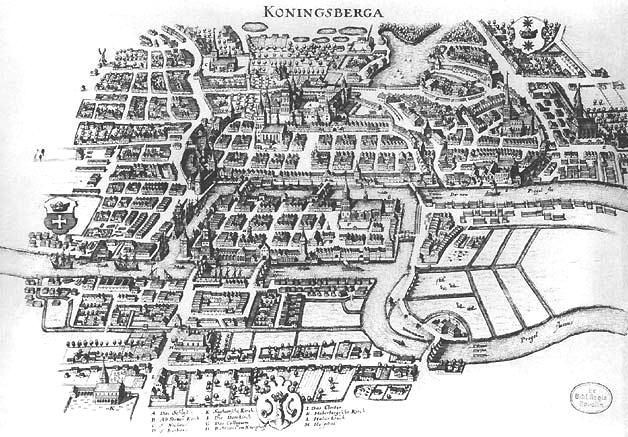
\includegraphics[height=6.5cm]{images/Koenigsberg,_Map_by_Merian-Erben_1652}}
\bigskip



\end{frame}

\begin{frame}\frametitle{Ein klassisches Problem}

Ein populäre Frage der Königsberger:\medskip

\anybox{strongyellow}{Gibt es einen Weg durch die Stadt, auf dem man jede der sieben Brücken von Königsberg genau einmal überquert?}\bigskip

Im Jahr 1735 beschäftigt sich Leonhard Euler (Mathematiker in Sankt Petersburg) mit der Frage \ldots\visible<2->{ und abstrahiert \ldots}\bigskip

\narrowcentering{%
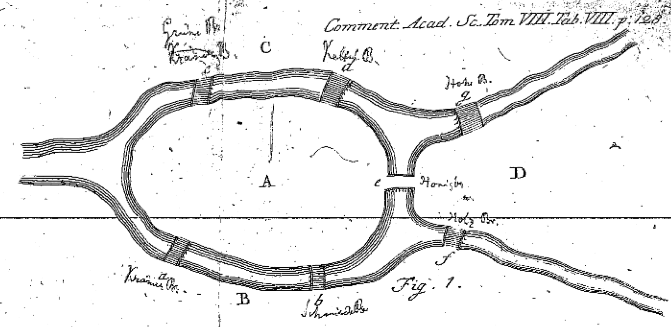
\includegraphics[height=2.5cm]{images/Koenigsberg,_Map_by_Euler.png}}
%
\pause
\begin{tikzpicture}[decoration=penciline, decorate]
% \path[use as bounding box] (-3.2,0) rectangle (3.5,-4); % add "draw" to see it
% \pgfmathsetseed{6571}
% \draw[help lines] (0,0) grid (5,5);
\node (A) [circle,draw=black,inner sep=1pt] at (0,0) {A};
\node (B) [circle,draw=black,inner sep=1pt] at (1,-1) {B};
\node (C) [circle,draw=black,inner sep=1pt] at (1,1) {C};
\node (D) [circle,draw=black,inner sep=1pt] at (2,0) {D};
% 
\draw[bend right] (A) edge (B);
\draw[bend left] (A) edge (B);
\draw (B) edge (D);
\draw (A) edge (D);
\draw (C) edge (D);
\draw[bend right] (A) edge (C);
\draw[bend left] (A) edge (C);
\end{tikzpicture}
\bigskip

\end{frame}

\begin{frame}\frametitle{Eulers Einsichten}

~\hspace{7.5cm}\ghost{
\begin{tikzpicture}[decoration=penciline, decorate,scale=0.8]
% \path[use as bounding box] (-3.2,0) rectangle (3.5,-4); % add "draw" to see it
% \pgfmathsetseed{6571}
% \draw[help lines] (0,0) grid (5,5);
\node (A) [circle,draw=black,inner sep=1pt] at (0,0) {A};
\node (B) [circle,draw=black,inner sep=1pt] at (1,-1) {B};
\node (C) [circle,draw=black,inner sep=1pt] at (1,1) {C};
\node (D) [circle,draw=black,inner sep=1pt] at (2,0) {D};
% 
\draw[bend right] (A) edge (B);
\draw[bend left] (A) edge (B);
\draw (B) edge (D);
\draw (A) edge (D);
\draw (C) edge (D);
\draw[bend right] (A) edge (C);
\draw[bend left] (A) edge (C);
\end{tikzpicture}}

\begin{itemize}
\item Lage der Brücken und Wege von einer Brücke zur nächsten sind egal\pause
\item Ein Pfad kann als Liste von Brücken dargestellt werden, aber es
gibt viele denkbare Listen ($7!=5040$)\pause
\item Wenn man $n$-mal auf einer Landmasse ankommt, dann muss man sie auch $n$-mal verlassen -- außer sie ist Start oder Ziel\pause
\item Daher muss jede Landmasse -- außer der Start und das Ziel -- eine gerade Zahl an
Brücken besitzen\pause
\end{itemize}
\redalert{$\leadsto$ Das Rätsel der Königsberger ist unlösbar}

\end{frame}

\begin{frame}\frametitle{Verallgemeinerung}

Euler legt damit den Grundstein für die Graphentheorie,
und definiert ein heute nach ihm benanntes Konzept:\bigskip

\defbox{Ein \redalert{Eulerpfad} ist ein Pfad in einem Graphen, 
der jede Kante genau einmal durchquert. Ein \redalert{Eulerkreis} ist ein
zyklischer Eulerpfad.}\bigskip\pause

Euler zeigte also:\medskip

\theobox{Satz (Euler): Ein Graph hat genau dann einen Eulerschen Pfad, wenn
er maximal zwei Knoten ungeraden Grades besitzt.}\bigskip\pause


\begin{tikzpicture}[decoration=penciline, decorate,scale=0.8]
\path[use as bounding box] (0,0) rectangle (1,1.5); % add "draw" to see it
\draw[fill=none,decorate,line width=0.3mm]
(0,0) -- (0,1);
\end{tikzpicture}\hfill
\begin{tikzpicture}[decoration=penciline, decorate,scale=0.8]
\path[use as bounding box] (0,0) rectangle (1,1.5); % add "draw" to see it
\draw[fill=none,decorate,line width=0.3mm]
(0,0) -- (0,1) -- (0.5,1.5);
\end{tikzpicture}\hfill
\begin{tikzpicture}[decoration=penciline, decorate,scale=0.8]
\path[use as bounding box] (0,0) rectangle (1,1.5); % add "draw" to see it
\draw[fill=none,decorate,line width=0.3mm]
(0,0) -- (0,1) -- (0.5,1.5) -- (1,1);
\end{tikzpicture}\hfill
\begin{tikzpicture}[decoration=penciline, decorate,scale=0.8]
\path[use as bounding box] (0,0) rectangle (1,1.5); % add "draw" to see it
\draw[fill=none,decorate,line width=0.3mm]
(0,0) -- (0,1) -- (0.5,1.5) -- (1,1) -- (0,1);
\end{tikzpicture}\hfill
\begin{tikzpicture}[decoration=penciline, decorate,scale=0.8]
\path[use as bounding box] (0,0) rectangle (1,1.5); % add "draw" to see it
\draw[fill=none,decorate,line width=0.3mm]
(0,0) -- (0,1) -- (0.5,1.5) -- (1,1) -- (0,1) -- (1,0);
\end{tikzpicture}\hfill
\begin{tikzpicture}[decoration=penciline, decorate,scale=0.8]
\path[use as bounding box] (0,0) rectangle (1,1.5); % add "draw" to see it
\draw[fill=none,decorate,line width=0.3mm]
(0,0) -- (0,1) -- (0.5,1.5) -- (1,1) -- (0,1) -- (1,0) -- (1,1);
\end{tikzpicture}\hfill
\begin{tikzpicture}[decoration=penciline, decorate,scale=0.8]
\path[use as bounding box] (0,0) rectangle (1,1.5); % add "draw" to see it
\draw[fill=none,decorate,line width=0.3mm]
(0,0) -- (0,1) -- (0.5,1.5) -- (1,1) -- (0,1) -- (1,0) -- (1,1) -- (0,0);
\end{tikzpicture}\hfill
\begin{tikzpicture}[decoration=penciline, decorate,scale=0.8]
\path[use as bounding box] (0,0) rectangle (1,1.5); % add "draw" to see it
\draw[fill=none,decorate,line width=0.3mm]
(0,0) -- (0,1) -- (0.5,1.5) -- (1,1) -- (0,1) -- (1,0) -- (1,1) -- (0,0) -- (1,0);
\end{tikzpicture}

\end{frame}

\begin{frame}\frametitle{Ein ähnliches Problem}

1859 publiziert der Physiker und Astronom Sir William Rowan Hamilton
ein Brettspiel. Es verkauft sich nicht gut, aber es liefert uns ein
weiteres Rätsel auf Graphen:

\defbox{Ein \redalert{Hamiltonpfad} ist ein Pfad in einem Graphen, 
der jeden Knoten genau einmal durchquert. Ein \redalert{Hamiltonkreis} ist ein
zyklischer Hamiltonpfad.}\bigskip\pause

Wie bei Eulerpfaden ist die naive Lösung sehr ineffizient, da man
alle (exponentiell viele) Pfade systematisch Durchprobieren muss.\bigskip\pause

Aber im Gegensatz zu Eulerpfaden hat bislang niemand eine elegante
einfache Lösung gefunden. Die meisten Experten glauben, dass es prinzipiell
keine effiziente Lösung geben kann.
\bigskip\pause

\narrowcentering{{\redalert{Kann man beweisen, dass es keine bessere Lösung gibt?}}}

\end{frame}

\begin{frame}\frametitle{Leicht oder schwer?}

\anybox{strongyellow}{\emph{Aufgabe:} Gegeben einen Graphen mit zwei Knoten $A$ und $B$, finde einen kürzesten Weg von $A$ nach $B$.}\pause\bigskip

\alert{Leicht!} Lösbar in polynomieller Zeit, z.B. mit Dijkstras Algorithmus
\bigskip\pause

\anybox{strongyellow}{\emph{Aufgabe:} Gegeben einen Graphen mit zwei Knoten $A$ und $B$, finde einen längsten Weg von $A$ nach $B$.}\pause\bigskip

\alert{Schwer!} Keine sub-exponentielle Lösung bekannt
\bigskip\pause

\medskip

\narrowcentering{{\redalert{Warum sind manche Probleme leicht und andere schwer?}}}\\[0.5ex]
\narrowcentering{\redalert{\tiny(obwohl sie sich auf den ersten Blick stark ähneln)}}

\end{frame}

\begin{frame}\frametitle{Einleitung}

\emph{Fragen:}
\begin{itemize}
\item Warum sind manche Probleme leicht und andere schwer?
\item Und sind sie wirklich schwer oder hatten wir nur bisher nicht die richtige Idee zu ihrer Lösung?
\end{itemize}\bigskip

\emph{Der Weg zu Antworten:}\smallskip

Ein Ziel der \alert{Komplexitätstheorie} ist die Unterteilung berechenbarer Probleme
entsprechend der Menge an Ressourcen, die zu ihrer Lösung nötig sind
\begin{itemize}
\item Unterteile Problem in Klassen gleicher "`Schwere"'
\item Entwickle Methoden zur Bestimmung der Komplexität eines Problems
\end{itemize}

\end{frame}

\sectionSlide{Beschränkung von Zeit und Raum}

\begin{frame}\frametitle{Turingmaschinen beschränken}

Wir wiederholen zunächst einige Grundlagen aus der Vorlesung Formale Systeme \ldots
\bigskip

TMs verwenden zwei Ressourcen, die man beschränken kann:
\begin{itemize}
\item \alert{Speicher:} die Zahl der verwendeten Speicherzellen
\item \alert{Zeit:} die Zahl der durchgeführten Berechnungsschritte
\end{itemize}\pause
Feste Schranken ergeben wenig Sinn (endliche Automaten)\\
\begin{enumerate}[$\leadsto$]
\item Schranken werden als Funktion in der Länge der Eingabe angegeben
\end{enumerate}
\bigskip

\examplebox{Beispiel: LBAs beschränken den verfügbaren Speicher auf die Anzahl der Symbole in der Eingabe.
Dies entspricht einer Funktion, welche die Länge $n$ der Eingabe auf den Maximalwert von $n$ Speicherzellen abbildet.}

\end{frame}

\begin{frame}\frametitle{Zur Erinnerung: $O$-Notation}

Die $O$-Notation (mit großem $O$!) charakterisiert Funktionen nach ihrem asymptotischen Verhalten und
versteckt lineare Faktoren.

\defbox{Für Funktionen $f,g: \mathbb{N}\to\mathbb{R}$ schreiben wir \redalert{$f\in O(g)$}
wenn gilt:\\[1ex]
%
\narrowcentering{Es gibt eine Zahl $c>0$ und eine Zahl $n_0\in\mathbb{N}$,}\\
\narrowcentering{so dass für jedes $n>n_0$ gilt: $f(n)\leq c\cdot g(n)$}\\[1ex]
%
Das bedeutet, $f$ wächst nicht wesentlich schneller als $g$.
}\pause

\emph{Notation 1:} Manchmal schreibt man statt $f\in O(g)$ auch $f=O(g)$ (allerdings ist $=$ dann eine
asymmetrische Relation).\medskip

\emph{Notation 2:} Manchmal schreibt man statt $f\in O(g)$ (oder $f=O(g)$) auch $f(n)\in O(g(n))$ (oder $f(n)=O(g(n))$).

\examplebox{Beispiele:
\begin{minipage}[t]{7cm}\vspace{-1.7ex}
\begin{itemize}
\item $(10 n^3+42 n^2 - n + 100)\in O(n^3)$
\item $(2^n + n^{2000})\in O(2^n)$
\item $2^{729}\in O(1)$
\end{itemize}
\end{minipage}
}

\end{frame}

\begin{frame}\frametitle{Schwestern der $O$-Notation}

\emph{Randbemerkung:} Es gibt neben der $O$-Notation noch eine Reihe weiterer
asymptotischer Notationen, die in der Informatik verwendet werden:\bigskip

\narrowcentering{
\begin{tabular}{ccc}
Notation & $C=\lim_{n\to\infty}\frac{f(n)}{g(n)}$ & Intuition \\\hline
$f\in O(g)$ & $C<\infty$ & "`$\,f\leq g$"' \\
$f\in \Omega(g)$ & $C>0$ & "`$\,f\geq g$"' \\
$f\in \Theta(g)$ & $0<C<\infty$ & "`$\,f= g$"' \\
$f\in o(g)$ & $C=0$ & "`$\,f<g$"' \\
$f\in \omega(g)$ & $C=\infty$ & "`$\,f>g$"' \\
\end{tabular}}

\end{frame}

\begin{frame}\frametitle{Schranken für Zeit und Raum}

Die $O$-Notation wird verwendet, um allgemeine Ressourcenschranken für TMs anzugeben.

\defbox{%
Sei $f:\mathbb{N}\to\mathbb{R}$ eine Funktion und $\Smach{M}$ eine Turingmaschine.
\begin{itemize}
\item $\Smach{M}$ heißt \redalert{$O(f)$-zeitbeschränkt} wenn es eine Funktion $g\in O(f)$ gibt, so
dass $\Smach{M}$ für eine beliebige Eingabe $w\in\Sigma^*$ nach maximal $g(|w|)$ Schritten anhält.
%
\item $\Smach{M}$ heißt \redalert{$O(f)$-speicherbeschränkt} wenn es eine Funktion $g\in O(f)$ gibt, so
dass $\Smach{M}$ für eine beliebige Eingabe $w\in\Sigma^*$ hält und zuvor maximal $g(|w|)$ Speicherzellen verwendet.
\end{itemize}
}\pause

\examplebox{Beispiel: Ein LBA entspricht einer $O(n)$-speicherbeschränkten \ghost{TM.}}

\examplebox{Beispiel: Eine naive Suche nach einem Eulerpfad wäre $O(n!)$-zeitbeschränkt, wenn die Zahl der Kanten $n$ nicht übersteigt.}

\end{frame}

\begin{frame}\frametitle{Lineare Faktoren}

Die $O$-Notation versteckt bei der Abschätzung der Laufzeit beliebig große konstante
Faktoren. Werden dadurch nicht zu viele unterschiedlich schwere Probleme in einen Topf
geworfen?\bigskip\pause

\alert{Nein.} Im Gegenteil: das TM-Modell der Berechnung kann konstante Faktoren
nicht unterscheiden, zumindest wenn man mehrere Bänder erlaubt:\medskip

\theobox{Satz (\alert{Linear Speedup Theorem}): 
Sei $\Smach{M}$ eine TM mit $k>1$ Bändern, die bei Eingaben der Länge $n$ nach maximal
$f(n)$ Schritten hält.
Dann gibt es für jede natürliche Zahl $c>0$ eine äquivalente $k$-Band TM
$\Smach{M}'$, die nach maximal $\frac{f(n)}{c}+n+2$ Schritten hält.
}\medskip\pause

\examplebox{Beispiel: Wenn ein Problem mit einer Zwei-Band-TM in $n^3$ Schritten gelöst werden kann, so ist das auch in $\frac{n^3}{1000000000}+n+2$ Schritten möglich.}

\end{frame}

\begin{frame}\frametitle{Linear Speedup Theorem: Beweis (1)}

\theobox{Satz (\alert{Linear Speedup Theorem}): 
Sei $\Smach{M}$ eine TM mit $k>1$ Bändern, die bei Eingaben der Länge $n$ nach maximal
$f(n)$ Schritten hält.
Dann gibt es für jede natürliche Zahl $c>0$ eine äquivalente $k$-Band TM
$\Smach{M}'$, die nach maximal $\frac{f(n)}{c}+n+2$ Schritten hält.
}

\pause\emph{Beweisskizze:} Wenn $\Smach{M}$ das Arbeitsalphabet $\Gamma$ hatte, dann verwenden wird für $\Smach{M}'$ das Arbeitsalphabet $\Gamma'=\Sigma\cup\Gamma^{6c}$.
\bigskip

Wir können Bandinhalte dadurch effizient kodieren:
\begin{itemize}
\item $\Smach{M}'$ liest die Eingabe und erzeugt eine kodierte Kopie auf Band 2
\item Dabei werden jeweils $6c$ Zeichen aus $\Sigma$ in eines aus $\Gamma^{6c}$ übersetzt
\item Diese Transkodierung benötigt $n+2$ Schritte
\end{itemize}


\end{frame}

\begin{frame}\frametitle{Linear Speedup Theorem: Beweis (2)}

\theobox{Satz (\alert{Linear Speedup Theorem}): 
Sei $\Smach{M}$ eine TM mit $k>1$ Bändern, die bei Eingaben der Länge $n$ nach maximal
$f(n)$ Schritten hält.
Dann gibt es für jede natürliche Zahl $c>0$ eine äquivalente $k$-Band TM
$\Smach{M}'$, die nach maximal $\frac{f(n)}{c}+n+2$ Schritten hält.
}

\emph{Beweisskizze:} Wir haben die Eingabe im Alphabet $\Gamma^{6c}$ kodiert.
\pause\medskip

Jetzt kann man $\Smach{M}$ simulieren:
\begin{itemize}
\item Lies (in vier Schritten) das $\Gamma^{6c}$-Symbol an den aktuellen $k$ Bandpositionen,
sowie jeweils links und rechts davon. 
\item Das Ergebnis und die genaue Bandposition von $\Smach{M}$ wird als Zustand gespeichert: wir verwenden dazu
$|Q\times\{1,\ldots,k\}\times \Gamma^{18c k}|$ zusätzliche Zustände
\item Simuliere (in zwei Schritten) die nächsten $6c$ Schritte von $\Smach{M}$
($\Smach{M}'$ verändert maximal das aktuelle Baldfeld und einen Nachbarn)
\end{itemize}
Ergebnis: Simulation von $6c$ $\Smach{M}$-Schritten und $6$ $\Smach{M}'$-Schritten.\qed
% \bigskip

\end{frame}

\begin{frame}\frametitle{Linear Speedup: Diskussion}

\alert{Kann jedes Programm beliebig schnell gemacht werden?}\bigskip\pause

In der Praxis: Nein
\begin{itemize}
\item Wirkprinzip Linear Speedup: kodiere mehr Information pro Bandfeld und verarbeite
diese auf einen Schlag mithilfe einer größeren Zustandsübergangstabelle
\item In der Praxis kann man nicht beliebig große Daten in einem Schritt lesen
\item In der Praxis kann man nicht beliebig komplexe Zustandsübergänge in konstanter
Zeit realisieren
\end{itemize}
\bigskip\pause

In der Theorie: Nein
\begin{itemize}
\item Wir interessieren uns für asymptotisches Verhalten bei beliebig wachsenden
	Eingaben
\item Lineare Faktoren machen meist nur bei relativ kleinen Werten einen Unterschied
\end{itemize}

\end{frame}

\sectionSlide{Wichtige Komplexitätsklassen}

\begin{frame}\frametitle{Zeit und Raum, deterministisch}

Beschränkte TMs können verwendet werden, um viele weitere Sprachklassen zu definieren.
\medskip

\defbox{Sei $f:\mathbb{N}\to\mathbb{R}$ eine Funktion.
\begin{itemize}
\item \redalert{\Scomplclass{DTIME}(f(n))} ist die Klasse aller Sprachen $\Slang{L}$, welche durch eine $O(f)$-zeitbeschränkte Turingmaschine entschieden werden können.
\item \redalert{\Scomplclass{DSPACE}(f(n))} ist die Klasse aller Sprachen $\Slang{L}$, welche durch eine $O(f)$-speicherbeschränkte Turingmaschine entschieden werden können.
\end{itemize}
}\pause

\examplebox{Beispiel: Die naive Suche nach Eulerpfaden kann in $\Scomplclass{DSPACE}(n)$ implementiert werden (Übung: wie?).}\pause

% \examplebox{Beispiel: $\Slang{SAT}\in\Scomplclass{DTIME}(2^n)$ und $\Slang{SAT}\in\Scomplclass{DSPACE}(n)$.}\pause

\examplebox{Beispiel: Das Halteproblem ist in keiner der Klassen $\Scomplclass{DTIME}(f(n))$ oder $\Scomplclass{DSPACE}(f(n))$, da es durch keine TM entschieden wird.}

\end{frame}

\begin{frame}\frametitle{Maschinenmodelle}

Es gibt viele unterschiedliche Versionen von deterministischen TMs und viele alternative Berechnungsmodelle (z.B. Mehrband-Maschinen und WHILE-Programme).\medskip

\anybox{purple}{Sind $\Scomplclass{DTIME}(f)$ und $\Scomplclass{DSPACE}(f)$ für jedes TM-Modell gleich?}\bigskip\pause

\emph{Antwort:} "`Nein, aber bei vielen typischen Variationen gibt es nur polynomielle Unterschiede."'\bigskip

\examplebox{Beispiel: Jede $O(f(n))$-zeitbeschränkte $k$-Band-TM kann durch eine $O(k\cdot f^2(n))$-zeitbeschränkte
1-Band TM simuliert werden (siehe Formale Systeme, Vorlesung 18). Einfacher gesagt: Der Verzicht auf mehrere Bänder verursacht maximal quadratische Zeitkosten ($k$ ist hier ein linearer Faktor).}

{\tiny \emph{Anmerkung:} Wir betrachten hier verschiedene Versionen deterministischer
Rechenmodelle. Zwischen DTMs und NTMs gibt es vermutlich
schon große (nicht-polynomielle) Unterschiede.

}

\end{frame}

\begin{frame}\frametitle{Kodierungsdetails}

Es gibt viele unterschiedliche Arten, wie Eingaben von Problemen als Wörter
kodiert werden können.\medskip

\anybox{purple}{Sind $\Scomplclass{DTIME}(f)$ und $\Scomplclass{DSPACE}(f)$ für jede Kodierung gleich?}\bigskip\pause

\emph{Antwort:} "`Nein, aber vernünftige Kodierungen unterscheiden sich voneinander
in der Regel nur polynomiell."'\bigskip

\examplebox{Beispiel: Ein Graph kann als Adjazenzmatrix kodiert werden ($O(n^2)$ Speicher) oder z.B. auch als Adjazenliste ($O(e\cdot \log v)$ Speicher für $e$ Kanten und $v$ Knoten). Letzteres ist deutlich effizienter für lichte Graphen, aber der Unterschied bleibt stets polynomiell.}\bigskip

\emph{Aber:} Wir werden Fälle sehen, in denen eine (besonders ineffiziente) Kodierung die Komplexität verändert.

\end{frame}

\begin{frame}\frametitle{Implementierungsdetails}

Es gibt viele unterschiedliche Arten um ein Problem praktisch zu lösen,
z.B. unter Verwendung spezifische Datenstrukturen.\\\smallskip

\anybox{purple}{Sind $\Scomplclass{DTIME}(f)$ und $\Scomplclass{DSPACE}(f)$ für verschiedene Implementierungsdetails gleich?}\pause\bigskip

\emph{Antwort:} "`Nein, aber die meisten Änderungen an der Implementierung haben bestenfalls polynomielle oder konstant-lineare Effekte."'\bigskip

% \examplebox{Beispiel: ? (konkrete Beispiele problematisch, da diese Effekte auch stark vom Maschinenmodell abhängen)}

% \begin{enumerate}[$\leadsto$]
% \item Es ist sinnvoll, \alert{noch allgemeinere Sprachklassen} zu betrachten, die auch gegenüber polynomiellen Änderungen der Ressourcen robust sind
% \end{enumerate}

\end{frame}

\begin{frame}\frametitle{Ist Komplexitätstheorie praktisch unmöglich?}

Die Klassen $\Scomplclass{DTIME}(f)$ und $\Scomplclass{DSPACE}(f)$
unterscheiden sich je nach
\begin{itemize}
\item Details des Maschinenmodells
\item Details der Eingabekodierung
\item Details der Implementierung
\end{itemize}

Eine exakte Bestimmung solcher Schranken ist oft sehr schwer.\medskip\pause

\examplebox{Beispiel: Ein naiver Algorithmus zur Matrixmultiplikation liegt in
$\Scomplclass{DTIME}(n^{\redalert{3}})$.
\only<-2>{~\\~\\~\\~\\}%
\only<3->{Seit Jahrzehnten sucher Forscher nach besseren
Lösungen:
$\Scomplclass{DTIME}(n^{\redalert{2.808}})$ [Strassen, 1969], 
$\Scomplclass{DTIME}(n^{\redalert{2.796}})$ [Pan, 1978],
$\Scomplclass{DTIME}(n^{\redalert{2.780}})$ [Bini et al., 1979],
$\Scomplclass{DTIME}(n^{\redalert{2.522}})$ [Schönhage, 1981],
$\Scomplclass{DTIME}(n^{\redalert{2.517}})$ [Romani, 1982],
$\Scomplclass{DTIME}(n^{\redalert{2.496}})$ [Coppersmith \& Winograd, 1981],
$\Scomplclass{DTIME}(n^{\redalert{2.479}})$ [Strassen, 1986],
$\Scomplclass{DTIME}(n^{\redalert{2.376}})$ [Coppersmith \& Winograd, 1990],
$\Scomplclass{DTIME}(n^{\redalert{2.374}})$ [Stothers, 2010] und
$\Scomplclass{DTIME}(n^{\redalert{2.373}})$ [Williams, 2011].}
\only<-3>{ \phantom{Vermutete} \phantom{optimale} \phantom{Lösung:} \phantom{$\Scomplclass{DTIME}(n^{\redalert{2}})$.}}%
\only<4->{\\ Vermutete optimale Lösung: $\Scomplclass{DTIME}(n^{\redalert{2}})$.}
}

\end{frame}

\begin{frame}\frametitle{Wie weiter?}


\emph{Problem:}
\begin{itemize}
\item Die exakte Bestimmung der Komplexität ist selbst bei einfachsten Algorithmen bisher nicht gelungen.
\item Selbst wenn sie gelänge ist sie von vielen detaillierten Annahmen abhängig, die praktische Computer eventuell nicht erfüllen.
\end{itemize}
\bigskip\pause

\emph{Lösung:}
\begin{itemize}
\item Wir betrachten \alert{noch allgemeinere Sprachklassen}, die auch gegenüber polynomiellen Änderungen der Ressourcen robust sind
\item Nachteil: Wir können nicht mehr zwischen $n$ und $n^{1000}$ unterscheiden
\item Vorteil: Wir müssen nicht mehr zwischen $n^{2.374}$ und $n^{2.373}$ unterscheiden
\end{itemize}

\end{frame}

\begin{frame}\frametitle{Wichtige Komplextitätsklassen}

Die wichtigen deterministischen Komplexitätsklassen fassen jeweils ganze Familien von
zeit- oder speicherbeschränkten Klassen zusammen. Wir erwähnen hier nur die praktisch wichtigsten:

{\footnotesize
\begin{align*}
\Scomplclass{P} = \Scomplclass{PTime} &= \bigcup_{d\geq 1} \Scomplclass{DTime}(n^d)
	& \text{\redalert{polynomielle Zeit}}
%   & \Scomplclass{NP} &= \bigcup_{k\geq 1} \Scomplclass{NTime}(n^k)
  \\[1ex]
\hspace{-1.5cm}\Scomplclass{Exp} = \Scomplclass{ExpTime} &= \bigcup_{d\geq 1} \Scomplclass{DTime}(2^{n^d})
    & \text{\redalert{exponentielle Zeit}${}^*$}
% %   & \Scomplclass{NExp} = \Scomplclass{NExpTime} &= \bigcup_{k\geq 1} \Scomplclass{NTime}(2^{n^k})
%   \\[1ex]
% \hspace{-1.5cm}\Scomplclass{2Exp} = \Scomplclass{2ExpTime} &= \bigcup_{d\geq 1} \Scomplclass{DTime}(2^{2^{n^d}})
% %   & \Scomplclass{N2Exp} = \Scomplclass{N2ExpTime} &= \bigcup_{k\geq 1} \Scomplclass{NTime}(2^{2^{n^k}})
% 	& \text{doppelt-exponentielle Zeit}
%   \\[1ex]
% \Scomplclass{E} = \Scomplclass{ETime} &= \bigcup_{d\geq 1} \Scomplclass{DTime}(2^{dn})
%    & \text{exp.\ Zeit mit linearem Exponent}
   \\[4ex]
\hspace{-1.5cm}\Scomplclass{L} = \Scomplclass{LogSpace} &= \Scomplclass{DSpace}(\log n)
%   & \Scomplclass{NL} = \Scomplclass{NLogSpace} &= \Scomplclass{NSpace}(\log n)
	& \text{\redalert{logarithmischer Speicher}}
  \\[1ex]
\Scomplclass{PSpace} &= \bigcup_{d\geq 1} \Scomplclass{DSpace}(n^d)
	& \text{\redalert{polynomieller Speicher}}
%   \\[1ex]
% \Scomplclass{ExpSpace} &= \bigcup_{d\geq 1} \Scomplclass{DSpace}(2^{n^d})
% 	& \text{exponentieller Speicher}
\end{align*}
}

\bigskip
{\tiny ${}^*$) Anmerkung: Dies ist die praktisch wichtigste Definition von "`exponentieller Zeit"'. Es gibt daneben auch
$\Scomplclass{E} = \Scomplclass{ETime} = \bigcup_{d\geq 1} \Scomplclass{DTime}(2^{dn})$ (exponentielle Zeit mit
linearem Exponenten).\\
}

\end{frame}

\begin{frame}\frametitle{\Scomplclass{LogSpace}? Wie soll das gehen?}

Für $n>1$ gilt \alert{$\log(n)<n$}. Auch beliebige lineare Faktoren können das nur für kleine $n$ kompensieren.\\
\medskip

Eine $O(\log(n))$-speicherbeschränkte TM darf also weniger Speicher verwenden als ihre Eingabe benötigt.
\alert{$\leadsto$ Wie soll das gehen?}
\bigskip\pause

\defbox{Man definiert \redalert{$O(\log(n))$-speicherbeschränkte Turingmaschinen} als besondere Mehrband-TMs:
\begin{itemize}
\item Das erste Band ist das \redalert{Eingabeband}. Es enthält die Eingabe und darf nur gelesen aber nicht beschrieben werden.
\item Das zweite Band ist das \redalert{Arbeitsband}. Es darf beliebig gelesen und beschrieben werden, aber es ist
auf $O(\log(n))$-Speicherzellen beschränkt.
\end{itemize}}

{\footnotesize
Das genügt zur Erkennung von Sprachen. Wenn die TM eine Ausgabe berechnen soll, dann wird dafür ein 
drittes \redalert{Ausgabeband} verwendet, auf dem man beliebig viele Zeichen einmalig schreiben aber nicht lesen kann.\\
}

\end{frame}

\begin{frame}\frametitle{Beziehungen der Komplexitätsklassen}

\alert{Eine wichtige Frage der Komplexitätstheorie ist, was man über die Beziehungen der
Komplexitätsklassen aussagen kann.}
\medskip\pause

Offensichtlich führen (asymptotisch) höhere Ressourcenschranken zu größeren Sprachklassen.
Oft ist aber nicht klar, ob man mit mehr Ressourcen auch wirklich mehr (oder einfach nur gleich viele) Probleme lösen kann. Bei
unseren Klassen ist das aber bekannt:\medskip

\theobox{Fakt: Es gilt $\Scomplclass{P}\subsetneq\Scomplclass{Exp}$ und
$\Scomplclass{LogSpace}\subsetneq\Scomplclass{PSpace}$.
}\medskip\pause

Weiterhin kann man Speicher mit Zeit in Beziehung bringen:
\begin{itemize}
\item In Zeit $n$ kann man nur $n$ Speicherzellen nutzen
\item Alle möglichen Konfigurationen auf $n$ Speicherzellen kann man in exponentieller Zeit (bezüglich $n$) berechnen
\end{itemize}

\theobox{Fakt: Es gilt $\Scomplclass{LogSpace}\subseteq\Scomplclass{P}\subseteq\Scomplclass{PSpace}\subseteq\Scomplclass{Exp}$.
}

\end{frame}

\begin{frame}\frametitle{Beispiele}

Unsere Klassen sind recht robust: Details der Implementierung haben oft keinen Einfluss
auf die Einordnung eines Problems.\\
\alert{Oft genügt eine Implementierungsskizze um zu zeigen, dass eine Sprache
in einer dieser Klassen liegt.}\pause

\examplebox{Beispiel: Eulers Methode um die Existenz von Eulerpfaden zu entscheiden,
kann in $\Scomplclass{LogSpace}$ implementiert werden: wir zählen die Kanten jedes Knotens 
und speichern die Zahl der Knoten ungerden Grades, jeweils binär.}\pause

\examplebox{Beispiel: Die Suche nach Hamilton-Pfaden ist in $\Scomplclass{ExpTime}$ aber auch in $\Scomplclass{PSpace}$.}\pause

\examplebox{Beispiel: Ein typisches Problem in $\Scomplclass{P}$ haben wir bereits in
der Vorlesug Formale Systeme kennengelernt: Erfüllbarkeit von propositionaler Horn-Logik. Unser Resolutionsalgorithmus
liefert allerdings keinen Hinweis auf Machbarkeit in $\Scomplclass{LogSpace}$.}\pause

\end{frame}

\begin{frame}\frametitle{Ressourcen nichtdeterministischer TMs}

Bei NTMs gibt es viele mögliche Berechnungspfade.\\
$\leadsto$ Welche Pfade meinen wir, wenn wir Ressourcen beschränken?\\\pause
~\hfill{\alert{-- Alle!}}
\medskip

\defbox{%
Sei $f:\mathbb{N}\to\mathbb{R}$ eine Funktion und $\Smach{M}$ eine nichtdeterministische \ghost{TM.}
\begin{itemize}
\item $\Smach{M}$ heißt \redalert{$O(f)$-zeitbeschränkt} wenn es eine Funktion $g\in O(f)$ gibt, so
dass $\Smach{M}$ für eine beliebige Eingabe $w\in\Sigma^*$ \alert{auf jedem Berechnungspfad} nach maximal $g(|w|)$ Schritten anhält.
%
\item $\Smach{M}$ heißt \redalert{$O(f)$-speicherbeschränkt} wenn es eine Funktion $g\in O(f)$ gibt, so
dass $\Smach{M}$ für eine beliebige Eingabe $w\in\Sigma^*$ hält und zuvor \alert{auf jedem Berechnungspfad} maximal $g(|w|)$ Speicherzellen verwendet.
\end{itemize}
}

Eine zeit- oder speicherbeschränkte NTM muss also auch auf erfolglosen Pfaden ("`falsch geratene Übergänge"') garantiert
innerhalb der Ressourcengrenzen halten.

\end{frame}

\begin{frame}\frametitle{Zeit und Raum, nichtdeterministisch}

Die entsprechenden Sprachklassen werden genau wie bei deterministischen TMs definiert:\medskip

\defbox{Sei $f:\mathbb{N}\to\mathbb{R}$ eine Funktion.
\begin{itemize}
\item \redalert{\Scomplclass{NTIME}(f(n))} ist die Klasse aller Sprachen $\Slang{L}$, welche durch eine $O(f)$-zeitbeschränkte NTM entschieden werden können.
\item \redalert{\Scomplclass{NSPACE}(f(n))} ist die Klasse aller Sprachen $\Slang{L}$, welche durch eine $O(f)$-speicherbeschränkte NTM entschieden werden können.
\end{itemize}
}%\pause
% 
% \examplebox{Beispiel: $\Slang{SAT}\in\Scomplclass{DTIME}(2^n)$ und $\Slang{SAT}\in\Scomplclass{DSPACE}(n)$.}\pause
% 
% \examplebox{Beispiel: Das Halteproblem ist in keiner der Klassen $\Scomplclass{DTIME}(f(n))$ oder $\Scomplclass{DSPACE}(f(n))$. Unentscheidbare Probleme benötigen uneingeschränkten Zugang zu beliebig vielen Ressourcen einer TM.}

\end{frame}


\begin{frame}\frametitle{Nichtdeterministische Komplextitätsklassen}

Auch hier beschränken wir uns auf einige wichtige Fälle:

{\footnotesize
\begin{align*}
\Scomplclass{NP} = \Scomplclass{NPTime} &= \bigcup_{d\geq 1} \Scomplclass{NTime}(n^d)
	& \text{\redalert{nichtdet. polynomielle Zeit}}
%   & \Scomplclass{NP} &= \bigcup_{k\geq 1} \Scomplclass{NTime}(n^k)
  \\[1ex]
\hspace{-1.5cm}\Scomplclass{NExp} = \Scomplclass{NExpTime} &= \bigcup_{d\geq 1} \Scomplclass{NTime}(2^{n^d})
    & \text{\redalert{nichtdet. exponentielle Zeit}}
% %   & \Scomplclass{NExp} = \Scomplclass{NExpTime} &= \bigcup_{k\geq 1} \Scomplclass{NTime}(2^{n^k})
%   \\[1ex]
% \hspace{-1.5cm}\Scomplclass{2Exp} = \Scomplclass{2ExpTime} &= \bigcup_{d\geq 1} \Scomplclass{DTime}(2^{2^{n^d}})
% %   & \Scomplclass{N2Exp} = \Scomplclass{N2ExpTime} &= \bigcup_{k\geq 1} \Scomplclass{NTime}(2^{2^{n^k}})
% 	& \text{doppelt-exponentielle Zeit}
%   \\[1ex]
% \Scomplclass{E} = \Scomplclass{ETime} &= \bigcup_{d\geq 1} \Scomplclass{DTime}(2^{dn})
%    & \text{exp.\ Zeit mit linearem Exponent}
   \\[4ex]
\hspace{-1.5cm}\Scomplclass{NL} = \Scomplclass{NLogSpace} &= \Scomplclass{NSpace}(\log n)
%   & \Scomplclass{NL} = \Scomplclass{NLogSpace} &= \Scomplclass{NSpace}(\log n)
	& \text{\redalert{nichtdet. logarithmischer Speicher}}
  \\[1ex]
\Scomplclass{NPSpace} &= \bigcup_{d\geq 1} \Scomplclass{NSpace}(n^d)
	& \text{\redalert{nichtdet. polynomieller Speicher}}
%   \\[1ex]
% \Scomplclass{ExpSpace} &= \bigcup_{d\geq 1} \Scomplclass{DSpace}(2^{n^d})
% 	& \text{exponentieller Speicher}
\end{align*}
}\pause

\examplebox{Beispiel: Die Existenz eines Hamiltonpfads ist in $\Scomplclass{NP}$ entscheidbar. Wenn ein Hamiltonpfad existiert, dann kann er in polynomieller Zeit
erraten und überprüft werden.
}

\end{frame}

\begin{frame}\frametitle{Deterministisch vs. nichtdeterministisch}

%
Welche Beziehungen haben diese Klassen zu anderen?\pause
{\footnotesize
\begin{itemize}
\item Die Beziehungen zwischen nichtdeterministischen Klassen sind analog zu denen im deterministischen Fall:\\[1ex]
\narrowcentering{$\Scomplclass{NL}\subseteq \Scomplclass{NP}\subseteq \Scomplclass{NPSpace}\subseteq \Scomplclass{NExp}$}
\pause
\item Eine DTM kann als NTM aufgefasst werden, d.h. die nichtdeterministischen Klassen sind immer stärker:\\[1ex]
\narrowcentering{$\Scomplclass{L}\subseteq \Scomplclass{NL}\qquad \Scomplclass{P}\subseteq \Scomplclass{NP}\qquad \Scomplclass{PSpace}\subseteq \Scomplclass{NPSpace}\qquad \Scomplclass{Exp}\subseteq \Scomplclass{NExp}$}
\pause
\item Man kann NTMs mit DTMs simulieren, aber das ist oft mit exponentiellen Mehrkosten verbunden (Vorlesung 19).
\pause
\item Der berühmte \alert{Satz von Savitch} besagt, dass speicherbeschränkte NTMs durch DTMs mit nur quadratischen Mehrkosten simuliert werden können. Insbesondere gilt damit $\Scomplclass{PSpace}= \Scomplclass{NPSpace}$.
\end{itemize}}
% Insgesamt ergeben sich folgende Beziehungen:
Zusammenfassung der wichtigsten bekannten Beziehungen:
\theobox{
\[\Scomplclass{L}\subseteq\Scomplclass{NL}\subseteq \Scomplclass{P}\subseteq\Scomplclass{NP}\subseteq\Scomplclass{PSpace}= \Scomplclass{NPSpace}\subseteq \Scomplclass{Exp}\subseteq \Scomplclass{NExp}\]
\vspace{-2.5ex}
}

\end{frame}

\begin{frame}\frametitle{Die Grenzen unseres Wissens}

Wir wissen:

\theobox{
\[\Scomplclass{L}\subseteq\Scomplclass{NL}\subseteq \Scomplclass{P}\subseteq\Scomplclass{NP}\subseteq\Scomplclass{PSpace}= \Scomplclass{NPSpace}\subseteq \Scomplclass{Exp}\subseteq \Scomplclass{NExp}\]
\vspace{-2.5ex}
}

\begin{itemize}
\item Wir wissen nicht, ob irgendeines dieser $\subseteq$ sogar $\subsetneq$ ist.
\item Insbesondere wissen wir nicht, ob $\Scomplclass{P}\subsetneq\Scomplclass{NP}$ oder $\Scomplclass{P}=\Scomplclass{NP}$.
\item Wir wissen nicht einmal, ob $\Scomplclass{L}\subsetneq\Scomplclass{NP}$ oder $\Scomplclass{L}=\Scomplclass{NP}$.
\end{itemize}\pause
Es wird aber vermutet, dass alle  $\subseteq$ eigentlich $\subsetneq$ sind.
% 
Bekannt ist das aber nur bei exponentiell großen Ressourcenunterschieden:

\theobox{Es gilt:
\begin{itemize}
\item $\Scomplclass{NL}\subsetneq\Scomplclass{PSpace}$
\item $\Scomplclass{P}\subsetneq\Scomplclass{Exp}$
\item $\Scomplclass{NP}\subsetneq\Scomplclass{NExp}$
\end{itemize}}

\end{frame}



\begin{frame}\frametitle{Zusammenfassung und Ausblick}

Die Komplexitätstheorie beschäfftigt sich mit der Klassifikation 
entscheidbarer Probleme nach ihrer Schwierigkeit\bigskip

Um robuste Ergebnisse zu erhalten, die nicht von Implementierungsdetails
abhängen, werden oft polynomielle Unterschiede in Kauf genommen\bigskip

Die wichtigsten Komplexitätsklassen sind
\[\Scomplclass{L}\subseteq\Scomplclass{NL}\subseteq \Scomplclass{P}\subseteq\Scomplclass{NP}\subseteq\Scomplclass{PSpace}= \Scomplclass{NPSpace}\subseteq \Scomplclass{Exp}\subseteq \Scomplclass{NExp}\]

\anybox{yellow}{
Was erwartet uns als nächstes?
\begin{itemize}
\item $\Scomplclass{P}$
\item $\Scomplclass{L}$
\item $\Scomplclass{NL}$
\end{itemize}
}

\end{frame}

% \begin{frame}[t]\frametitle{Literatur und Bildrechte}
% 
% \alert{Literatur}\bigskip
% 
% \begin{itemize}
% \item Richard J. Lorentz:
% \emph{Creating Difficult Instances of the Post Correspondence Problem.}
% Computers and Games 2000: 214--228
% \item John J. O'Connor, Edmund F. Robertson: \emph{Emil Leon Post.} MacTutor History of Mathematics archive, University of St Andrews. \url{http://www-history.mcs.st-andrews.ac.uk/Biographies/Post.html}
% \end{itemize}
% 
% \bigskip\bigskip
% 
% \alert{Bildrechte}\bigskip
% 
% Folie \ref{frame_post}: gemeinfrei
% 
% \end{frame}


\end{document}